\documentclass[english,serif,mathserif,xcolor=pdftex,dvipsnames,table]{beamer}

\usepackage[T1]{fontenc}
\usepackage[utf8]{inputenc}

\usetheme[informal]{s3it}
\usepackage{s3it}

\title[7. Dictionaries]{%
  A Short and Incomplete Introduction to Python
}
\subtitle{\bfseries Part 7: \texttt{dict}s and other data structures}
\author[R.~Murri]{%
  \textbf{Riccardo Murri} \texttt{<riccardo.murri@uzh.ch>}, \\
  Sergio Maffioletti \texttt{<sergio.maffioletti@uzh.ch>}
  \\
  S3IT: Services and Support for Science IT,
  \\
  University of Zurich
}
\date{January 18/21, 2019}


\begin{document}

% title frame
\maketitle


\part{Dictionaries}

%%% dictionaries

\begin{frame}[fragile]
  \frametitle{Dictionaries}
  The \texttt{dict} type implements a key/value mapping:
\begin{lstlisting}
>>> D = { }  # empty dict
>>> D['a'] = 1
>>> D[2] = 'b'
>>> D
{'a': 1, 2: 'b'}
\end{lstlisting}

\+
  Dictionaries can be created and initialized using the following syntax:
\begin{lstlisting}
>>> D = { 'a':1, 2:'b' }
>>> D['a']
1
\end{lstlisting}
\end{frame}

\begin{frame}[fragile]
  The \texttt{for} statement can be used to loop over keys of a dictionary:
  \+
  \begin{columns}[c]
    \begin{column}{0.5\textwidth}
\begin{lstlisting}
>>> D = { 'a':1, 'b':2 }
>>> for val in ~\HL{D.keys()}~:
...   print(val)
'a'
'b'
\end{lstlisting}
    \end{column}
    \begin{column}{0.4\textwidth}
      \raggedleft
      Loop over dictionary~\emph{keys}.

      \emph{The \texttt{.keys()} part can be omitted, as it's the
        default!}
    \end{column}
  \end{columns}
\end{frame}


\begin{frame}[fragile]
  If you want to loop over dictionary \emph{values}, you have to
  explicitly request it.

  \+
  \begin{columns}[c]
    \begin{column}{0.5\textwidth}
\begin{lstlisting}
>>> D = { 'a':1, 'b':2 }
>>> for val in ~\HL{D.values()}~:
...   print(val)
1
2
\end{lstlisting}
    \end{column}
    \begin{column}{0.4\textwidth}
      \raggedleft
      Loop over dictionary~\emph{values}

      \emph{The \texttt{.values()} cannot be omitted!}
    \end{column}
  \end{columns}
\end{frame}


\begin{frame}[fragile]
  Finally, you can request keys \emph{and} corresponding values with
  the \texttt{.items()} iterator:

  \+
  \begin{columns}[c]
    \begin{column}{0.5\textwidth}
\begin{lstlisting}
>>> D = { 'a':1, 'b':2 }
>>> for key, val in ~\HL{D.items()}~:
...   print(key, '=>', val)
a=>1
b=>2
\end{lstlisting}
    \end{column}
    \begin{column}{0.4\textwidth}
      \raggedleft
      Loop over dictionary~\emph{items}.

      \+
      Note the syntax for multiple-assignment!
    \end{column}
  \end{columns}
\end{frame}


\begin{frame}[fragile]
  \frametitle{The `{\ttfamily\bfseries in}' operator (2)}

  Use the \lstinline|in| operator to test for presence of an item in a
  collection.

  \begin{describe}{\lstinline|x in D| \\ \lstinline|x in D.keys()|}
    Evaluates to \texttt{True} if \lstinline|x| is equal to a \emph{key}
    in the \lstinline|D| dictionary.
  \end{describe}

  \begin{describe}{\lstinline|x in D.values()|}
    Evaluates to \texttt{True} if \lstinline|x| is equal to a \emph{value}
    in the \lstinline|D| dictionary.
  \end{describe}

\end{frame}


\begin{frame}[fragile]
\begin{exercise*}[7.A]
    Write a function \lstinline|wordcount(filename)| that reads a text
    file and returns a dictionary, mapping words into occurrences
    (disregarding case) of that word in the text.

    \+ For example, using the
    \href{https://github.com/riccardomurri/python-for-science-intro/blob/master/exercises/lipsum.txt}{lipsum.txt}
    file:
    \begin{lstlisting}
>>> wordcount('lipsum.txt')
{'and': 3, 'model': 1, 'more-or-less': 1,
 'letters': 1, ~{\em [...]}~
    \end{lstlisting}

    \+ For the purposes of this
    exercise, a ``word'' is defined as a sequence of letters and the
    character ``-'', i.e., ``e-mail'' and ``more-or-less'' should both
    be counted as a single word.
  \end{exercise*}
\end{frame}


\part{Bar plots}

\begin{frame}[fragile]
  \frametitle{Bar plots, I}
  \small
  Seaborn's \texttt{barplot()} function can be used \\ to draw bar plots.

  \+
\begin{semiverbatim}\small
\In \,\,x = [0, 1, 2, 3, 4, 5]
\In \,\,y = [3, 1, 2, 4, 0, 5]
\In \HL{seaborn.barplot(x, y)}
\end{semiverbatim}
  \begin{center}
    \includegraphics[height=0.50\textheight]{fig/barplot0.pdf}
  \end{center}
\end{frame}


\begin{frame}[fragile]
  \frametitle{Bar plots, II}
  \small
  \only<1>{%
    An additional argument \texttt{orient=...} can be used to give:
    \begin{itemize}
    \item   vertical orientation (\texttt{orient='v'}, default), \emph{or}
    \item horizontal (\texttt{orient='h'}).
    \end{itemize}
  }%
  \only<2>{%
    Note that the role of \texttt{x} and \texttt{y} parameters is
    \emph{reversed} in horizontal plots: \texttt{x} is the size of bars,
    \texttt{y} is the labels.
  }%

\begin{semiverbatim}\small
\In \,\,x = [0, 1, 2, 3, 4, 5]
\In \,\,y = [3, 1, 2, 4, 0, 5]
\In \HL{seaborn.barplot(y, x, orient='h')}
\end{semiverbatim}
  \begin{center}
    \includegraphics[height=0.50\textheight]{fig/barplot0.pdf}
  \end{center}
\end{frame}


\begin{frame}[fragile]
  \frametitle{Bar plots, III}
  \small

    Arguments \texttt{x} and \texttt{y} can be Python lists or NumPy arrays, as usual.

    \+
    Another variant (available in all Seaborn plotting functions)
    is to pass a PanDas \texttt{DataFrame} object with the
    \texttt{data=...} argument, and then \texttt{x} and \texttt{y}
    become names of columns in the data frame.

    \+
\begin{semiverbatim}
seaborn.barplot(data=csv, x="word", y="frequency")
\end{semiverbatim}
\end{frame}


\part{References and copies}

\begin{frame}[fragile]
  \frametitle{Variables are names for values}

  \textbf{Python variables are just ``names'' given to values.}

  \+
  This allows you to \emph{reference} the string \texttt{'Python'}
  by the \emph{name} \texttt{a}.  But also by another name \texttt{b}:

  \+
  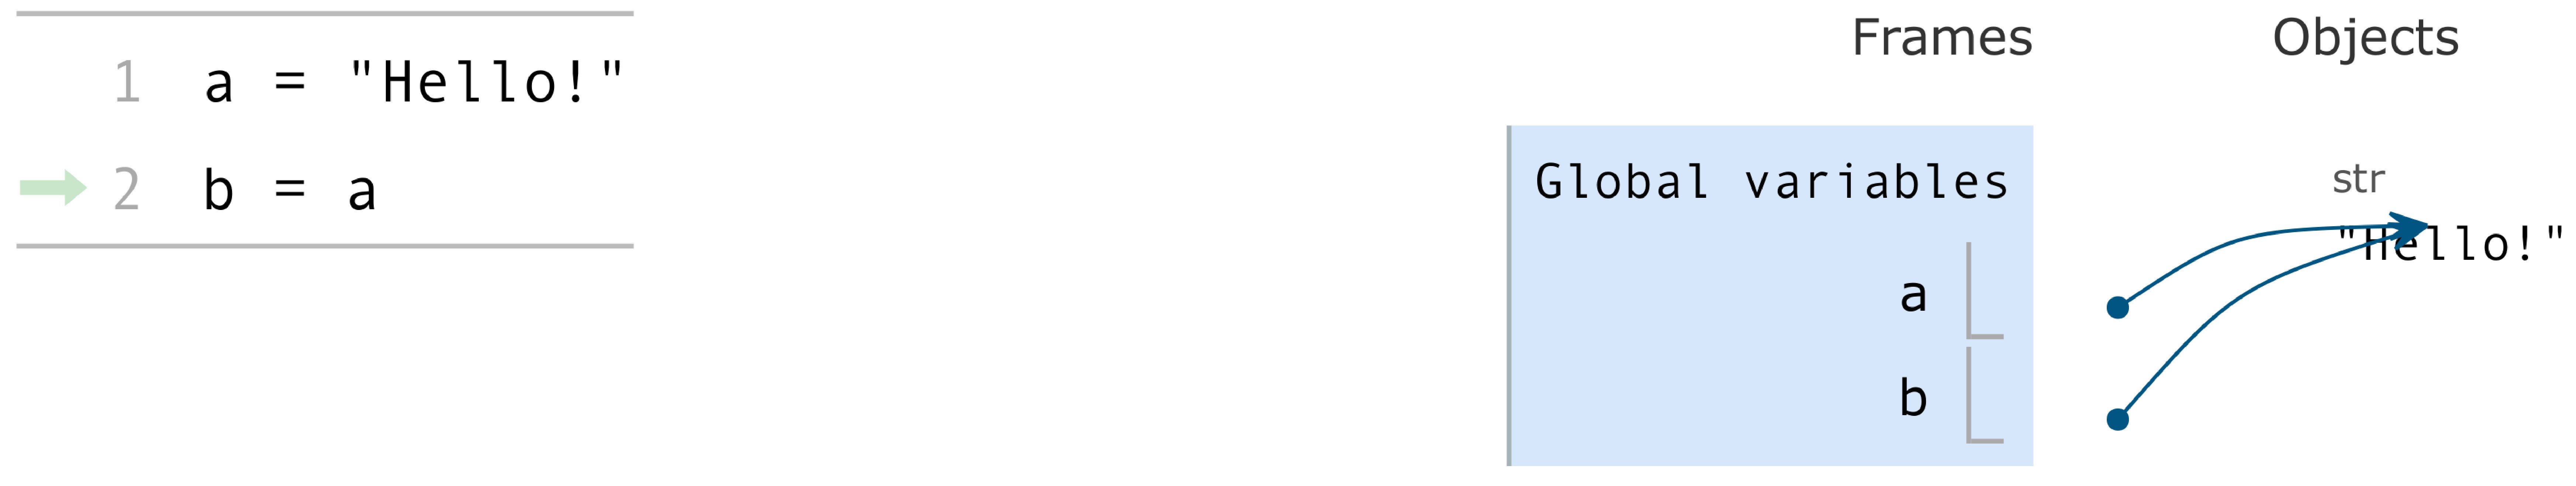
\includegraphics[width=1.00\linewidth]{fig/a=b.pdf}

  \+
  The \emph{same} object can be given many names!

  \+
  \begin{seealso}
    \scriptsize \url{http://excess.org/article/2014/04/bar-foo/}
  \end{seealso}
\end{frame}


\begin{frame}[fragile]
  \frametitle{The \texttt{is} operator}

  The \texttt{is} operator allows you to test whether two names refer
  to the same object:
  \begin{columns}
    \begin{column}{0.3\linewidth}
\begin{lstlisting}
>>> a = 1
>>> b = 1
>>> a == b
True
>>> a is b
True
\end{lstlisting}
    \end{column}
    \begin{column}{0.3\linewidth}
\begin{lstlisting}
>>> a = ''
>>> b = ""
>>> a == b
True
>>> a is b
True
\end{lstlisting}
    \end{column}
    \begin{column}{0.3\linewidth}
\begin{lstlisting}
>>> a = list()
>>> b = list()
>>> a == b
True
>>> a is b
False
\end{lstlisting}
    \end{column}
  \end{columns}

\end{frame}


\begin{frame}[fragile]
  \frametitle{All variables are references}

  In Python, \textbf{all objects are ever passed by reference}.

  \+
  In particular, \textbf{variables always store a reference to an
    object}, never a copy!

  \+
  Hence, you have to be careful when modifying objects:
\begin{lstlisting}
>>> a = [1,2,3]
>>> b = a
>>> b.remove(2)
>>> print(a)
\end{lstlisting}
  \only<1>{%
\vspace{-1.5em}
\begin{semiverbatim}
\emph{???}
\end{semiverbatim}
    \begin{center}
      \textbf{Q}: How many items are in the \texttt{a} list now?
    \end{center}
  }%
  \only<2>{%
\vspace{-1.5em}
\begin{semiverbatim}
[1, 3]
\end{semiverbatim}

   \+
   \href{http://tinyurl.com/cq3tcab}{Run this example} in the
   \href{http://pythontutor.com/}{Online Python Tutor} to better
   understand what's going on.

   \+
   {\small \em
     This applies particularly for variables that capture the arguments
     to a function call!}
}%
\end{frame}


\begin{frame}[fragile]
  \frametitle{All variables are references (demo)}

  \href{http://www.pythontutor.com/}{www.pythontutor.com}
  \+

  \only<1>{\includegraphics[width=1.2\textheight]{fig/t1_screenshot_1.png}}
  \only<2>{\includegraphics[width=1.2\textheight]{fig/t1_screenshot_2.png}}
  \only<3>{\includegraphics[width=1.2\textheight]{fig/t1_screenshot_3.png}}
  \only<4>{\includegraphics[width=1.2\textheight]{fig/t1_screenshot_4.png}}

\end{frame}


\subsection{Making copies}

\begin{frame}[fragile]
  \frametitle{How to copy an object? (0)}
  \begin{lstlisting}
>>> a = [1, 2]
>>> b = a
>>> b.remove(1)
>>> print(b)
[2]
>>> print(a)
[2]
  \end{lstlisting}
\end{frame}


\begin{frame}[fragile]
  \frametitle{How to copy an object? (1)}
  \begin{lstlisting}
>>> from copy import copy
>>> a = [1, 2]
>>> b = copy(a)
>>> b.remove(1)
>>> print(b)
[2]
>>> print(a)
[1, 2]
  \end{lstlisting}
\end{frame}


\begin{frame}[fragile]
  \frametitle{How to copy an object? (2)}
Note that \texttt{copy.copy} makes a \emph{shallow} copy:
  \begin{lstlisting}
>>> D = { 'a':[1,2], 'b':3 }
>>> print(D['a'])
[1, 2]
>>> E = copy(D)
>>> print(E)
{ 'a':[1, 2], 'b':3 }
>>> E['a'].remove(1)
>>> print(D['a'])
[2]
  \end{lstlisting}
\end{frame}


\begin{frame}[fragile]
  \frametitle{How to copy an object? (3)}
  To make a copy of nested data structures, \\
  you need \texttt{copy.deepcopy}:
\begin{lstlisting}
>>> from copy import deepcopy
>>> D = { 'a':[1,2], 'b':3 }
>>> print(D['a'])
[1, 2]
>>> E = deepcopy(D)
>>> print(E)
{ 'a':[1, 2], 'b':3 }
>>> E['a'].remove(1)
>>> print(D['a'])
[1, 2]
>>> print(E['a'])
[2]
  \end{lstlisting}
\end{frame}


\part{Appendix}

\subsection{Mutable vs immutable}

\begin{frame}[fragile]
  \frametitle{Mutable vs Immutable}
  Some objects (e.g., \texttt{tuple}, \texttt{int}, \texttt{str})
  are \emph{immutable} and cannot be modified.
\begin{lstlisting}
>>> S = 'UZH'
>>> S[2] = 'G'
Traceback (most recent call last):
  File "<stdin>", line 1, in <module>
TypeError: 'str' object does not support item assignment
\end{lstlisting}


  \+
  \texttt{list}, \texttt{dict}, \texttt{set} and user-defined objects
  are \emph{mutable} and can be modified in-place.
\end{frame}

\begin{frame}[fragile]
  \frametitle{Dictionary, sets and mutable objects}

  Not all objects can be used as dictionary \emph{keys} or items in a
  set:
  \begin{itemize}
    \item
      \textit{Immutable} objects \textbf{can be} used as \texttt{dict} keys or set items.
    \item
      \textit{Mutable} objects  \textbf{cannot be} used as \texttt{dict} keys or set items.
    \end{itemize}

    \+
    {\footnotesize
      (Explanation for the technically savvy: a dictionary is
      essentially a \href{http://en.wikipedia.org/wiki/Hash_table}{Hash
        Table}, therefore keys of a dictionary must be \textit{hashable}
      objects.  If objects were allowed to mutate, their hash value
      would change too and we would lose the mapping.)}
\end{frame}


\part{Other containers}
\begin{frame}
  \frametitle{Other containers}

  The following builtin containers are always available:
  \begin{description}
  \item[dict] \textit{mutable} key/value mapping.
  \item[set] \textit{mutable}, unordered set of \textit{unique} elements.
  \item[frozenset] \textit{immutable}, unordered set of
    \textit{unique} elements.
  \end{description}

  \pause
  Other specialized containers are available in the
  \texttt{collections} module:

  \begin{description}
  \item[dequeue] a generalization of stacks and queues
  \item[namedtuple] similar to a tuple, but allows you to access the
    elements \textit{by name}
  \item[OrderedDict] dictionary that remembers the order that the
    items were inserted.
  \end{description}
\end{frame}


\end{document}

%%% Local Variables:
%%% mode: latex
%%% TeX-master: t
%%% End:
